
\documentclass[conference]{IEEEtran}
% *** CITATION PACKAGES ***
%
\usepackage{cite}

% *** GRAPHICS RELATED PACKAGES ***
%
\usepackage[pdftex]{graphicx}
\graphicspath{./figures/}

% *** SUBFIGURE PACKAGES ***
%\ifCLASSOPTIONcompsoc
%  \usepackage[caption=false,font=normalsize,labelfont=sf,textfont=sf]{subfig}
%\else
%  \usepackage[caption=false,font=footnotesize]{subfig}
%\fi

\usepackage{url}


\begin{document}

\title{Cognitive Architecture for Mutual Modelling}


% author names and affiliations
% use a multiple column layout for up to three different
% affiliations
\author{\IEEEauthorblockN{Alexis Jacq$^{1,2}$, Wafa Johal$^1$, Pierre Dillenbourg$^1$, Ana Paiva$^2$}
\IEEEauthorblockA{
$^1$CHILI Lab, \'Ecole Polytechnique F\'ed\'erale de Lausanne (EPFL), Lausanne,
Switzerland}
\IEEEauthorblockA{
$^2$INESC-ID \& Instituto Superior T\'{e}cnico, University of Lisbon, Portugal
}
}



\maketitle

% As a general rule, do not put math, special symbols or citations
% in the abstract
\begin{abstract}
In an educational scenario, learners and teacher are able to understand each other. 
%For instance, learners share their knowledge and they must adapt their behaviour in order to make sure they are understood by others. 
Learners display behaviours in order to show their understanding and teachers adapt in order to make sure that the learners' knowledge is the required one. 
This ability requires a model of their own mental states perceived by others.
%For instance, did the learner saw that the teacher saw that the learner misunderstood the aim of the task?

In this paper, we discuss of the importance of a cognitive architecture enabling second-order Mutual Modelling for Human-Robot Interaction in educative contexts.


\end{abstract}

% no keywords




% For peer review papers, you can put extra information on the cover
% page as needed:
%e \ifCLASSOPTIONpeerreview
% \begin{center} \bfseries EDICS Category: 3-BBND \end{center}
% \fi
%
% For peerreview papers, this IEEEtran command inserts a page break and
% creates the second title. It will be ignored for other modes.
\IEEEpeerreviewmaketitle



\section{Introduction}
%Why should you use cognitive architectures - how would they benefit your research as a theoretical framework, a tool and/or a methodology?
%
%Should cognitive architectures for social interaction be inspired and/or limited by models of human cognition?
%
%What are the functional requirements for a cognitive architecture to support social interaction?
%
%How the requirements for social interaction would inform your choice of the fundamental computational structures of the architecture (e.g. symbolic, sub-symbolic, hybrid, ...)?
%
%
%Can you devise a social interaction scenario that current cognitive architectures would likely fail, and why?
%
%
%Robots present as assistant in various domains health, rescue, education
%
%Robots are brought o be in social interaction with humans.
%Necessity to behave in an acceptable and understandable manner by the user.

%%%% ToM

A social robot is brought to interact with humans. The quality of this interaction depends on its ability to behave in an acceptable and understandable manner by the user. Hence the importance for a robot to take care of his image: how much it is perceived as an automatic and boring agent, or contrariwise as a surprising and intelligent character. If the robot is able to detect this perception of itself, it can adapt its behaviour in order to be understood: ``you think I am sad while I am happy, I want you to understand that I am happy". In a collaborative context, where knowledge must be shared, agents must exhibit that they are acquiring the shared information with an immediate behaviour: ``I look what you are showing to me, do you see I am looking what you are showing, do you think I am paying attention to your explanation ?"; ``I have understood your idea, do you understand I have understood ?". We have different strategies to exhibit understanding or to repair a miss-understanding. As an example, if someone is talking about a visual object, we alternatively gaze at the object and at the person to make sure he saw we gazed at the object. Or if we detect that the other have not understood a gesture (e.g. pointing an object) we probably exaggerate the gesture.

Developed by Baron-Cohen and Leslie~\cite{baron1985does}, the Theory of Mind (ToM) describes the ability to attribute mental states and knowledge to others. In interaction, humans are permanently collecting and analysing huge quantity of information to stay aware of emotions, goals and understandings of their fellows. In this work, we focus on a generalization of this notion: Mutual Modelling characterizes the effort of one agent to model the mental state of another one~\cite{dillenbourg1999you}. 

Until now, the work conduced by the Human-Robot Interaction (HRI) community to develop mutual modelling abilities in robots was limited to a first level of modelling (see Related Work section~\ref{rw}). Higher levels require the ability to recursively attribute a theory of mind to other agent (\textit{I think that you think that} ...) and their application to HRI remains unexplored. However, a knowledge of oneself perceived by others is necessary to adapt a behaviour to keep mutual understandings. Without such a reflection it is possible to try collaborations, but no immediate feedbacks of success are given. If the trial has failed it is impossible to guess it and to repair it. 

%%%% CoWriter
% improve transition
% elgaguer

An important challenge of social robotics is to provide assistance in education. 
The ability of robots to support adaptive and repetitive task can be valuable in a learning interaction.
The CoWriter Project~\cite{Hood,jacq2016building} introduces a new approach to help children with difficulties to learn handwriting. 
Based on the \emph{learning by teaching} paradigm, the goal of the project is not only to help children with their handwriting but mainly to improve their self-confidence and motivation in practising handwriting.

\emph{Learning by teaching} engages students to conduct the activity in the role of the teachers in order to support their learning process. 
This  paradigm is known to produce motivational, meta-cognitive and educational benefits in a range of disciplines~\cite{Rohrbeck2003}. 
The CoWriter project is the first application of learning by teaching approach to handwriting.

The effectiveness of this learning by teaching activity is built on the ``prot\'eg\'e effect'': the teacher feels responsible for his student, commits
to the student's success and possibly experiences student's failure as his own
failure to teach. 
The main idea is to promote the child's extrinsic motivation to write letters (he will do it in order to help his ``prot\'eg\'e" robot) and to reinforce the self-esteem of the child (he plays the teacher and the robot actually progresses).

In that context, the robot needs to pretend enough difficulties to motivate the child to help it. 
This pretending strongly depends on the perception of the robot by the child: the displayed behaviours (gestures, gazes and sounds) by the robot, the initial level and learning speed of the robot must match with what the child imagines of a ``robot in difficulty".
In order to adapt to the child, the robot needs then to have a model of how it is perceived by the child. On the other side, the child builds also a model of the robot's difficulties and attitude. 
This mutual-modelling is primordial in order to have mutual understanding and fluid interaction between learner and teacher. 



\section{Related works}

A large amount of fields have introduced frameworks to describe mutual modelling ability~\cite{lemaignan2015mutual}. 
In developmental psychology Flavell~\cite{flavell1990developmental} denotes two different levels of perspective taking: the \textit{cognitive connection} (I see, I hear, I want, I like...) and \textit{mental representation} (what other agents feel, hear, want...).

From a computational perspective, Epistemic logic describes knowledges and beliefs shared by agents. This framework enables consideration of infinite-level of mutual modelling. It defines a \textit{shared-knowledge} (all the agents of a group know \textbf{X}) and a \textit{common-knowledge} (all the agents of a group know \textbf{X}, and know that all the agent know \textbf{X}, and know that all the agents know that all the agents know \textbf{X}, \dots.)~\cite{hendricks2008epistemic}. 

Mutual modelling has also been studied through educational contexts. Roschelle and Teasley~\cite{roschelle1995construction} suggested that collaborative learning requires a \textit{shared understanding} of the task and of the shared information to solve it. 
The term ``mutual modelling" was introduced in Computer-Supported Collaborative Learning (CSCL) by Dillenbourg~\cite{dillenbourg1999you}. It focused on knowledge states of agents. Dillenbourg developed in \cite{sangin2007partner} a computational framework to represent mutual modelling situations.

However, HRI research has not, until now, explored the whole potential of mutual modelling. In \cite{scassellati2002theory}, Scassellati supported the importance of Leslie's and Baron-Cohen's theory of mind to be implemented as an ability for robots. 
He focused his work on attention and perceptual processes (face detection or colour saliency detection). Thereafter, some works (including Breazeal~\cite{breazeal2006using}, Trafton~\cite{Trafton2005}, Ros~\cite{Ros2010} and Lemaignan~\cite{lemaignan2012thesis}) were conduced to implement Flavell's first level of perspective taking~\cite{flavell1977development} (``\textit{I see (you do not see the book)}"), ability that is still limited to visual perception. 

Breazeal~\cite{breazeal2009embodied} and Warnier~\cite{warnier2012when} reproduced the Sally and Anne's test of Wimmer~\cite{wimmer1983beliefs} with robots able to perform visual perspective taking. The robot was able to infer the knowledge of a human given the historic of his visual experience. 

In \cite{lemaignan2016realtime}, Lemaignan implemented a system that compute in real-time the visual field of agents and estimate which objects are looked at. This time, the robot is not just aware of what \textit{can be seen} by agents, but it perceives what \textit{is currentl
y looked at}. Lemaignan used this system to measure Sharma's \textit{with-me-ness}~\cite{sharma2014me}, visual commitment based on expected focus of attention in an activity. 
\section{MM-based reasoning}

We must make a distinction between architectures that performs mutual modelling and simple cognitive architectures (that does not model other agents) in order to avoid miss-understandings and Russel's paradoxes. Let's call \textit{basic} such a simple architecture and \textit{MM-based} the mutual modelling ones. 

%\subsection{Representation of models}
A first intuition for mutual modelling is to assume that all agents have the same basic architecture. In [], Breazeal show a MM-based reasoning where the robot uses its own basic architecture to model other agents. We can imagine a second level of modelling where a robot uses its MM-based architecture to model the other agent. But that creates an infinite recursive loop: the agent then models the robot that models the agent etc. Another reason to avoid a recursive approach is that different agent must have different behaviours: in similar situations, they will not necessary take similar decisions. 

We propose a different approach of modelling, where we define two orders of agents: the \textit{first-order-agents} concern direct representations of agents by the robot (for example the child), while the \textit{second-order-agents} concern the representation of agents by agents (for example the robot-perceived-by-the-child). 
To model second-order-agent like the robot-perceived-by-the-child will help to model how the child perceives the robot, e.g. to make sure the child understand that the robot is learning from his demonstrations. 
We can as well define \textit{$n^{\textit{th}}$-order} agents with higher level of theory of mind. But taking into account high levels of mutual modelling would be difficult to process in real time. Unlike the epistemic logic, our proposed framework will not take into account infinite regress~\cite{clark1991grounding} of mutual modelling.

All sensors (cameras, micros, motor positions ... and in the case of CoWriter the tablet's inputs) are used to
perceive information about the physical behaviour of agents. We call \textit{perceived variables} all the measurable quantities or qualities that provide such information (position in space, gaze's direction, speeches, movements, facial expressions ...). Thus, each agent's model is associated with a set of perceived variables that describes his physical behaviour.

But emotional states of agents cannot be directly measured directly from sensors. We call \textit{abstract variables} all the quantities or qualities that describe the mental state of an agent. Abstract variables are deduced from the dynamic of perceived variables. As an example, if the robot shows an object by pointing it with its arm, it expects the child to look at the object. If then the child looks at the hand of the robot, the robot can deduce that the child has not understood the meaning of its gesture. The perceived variables are the robot's gesture and the gaze direction of the child. The deduced abstract variable is the understanding of the gesture by the child. 

A model of an agent is the set of all the values of the perceived or abstract variables associated with this model. Since the values of variables are likely to change with the time, the models must be dynamic.

%\subsection{Reasoning}

In order to deduce the values of abstract variables (that can't be obtained from direct perception),
we propose to build a Bayesian model based on the knowledge from perceived variables. 
The choice of a probabilist approach instead of a symbolic approach comes from the errors in the perception of the robot: knowledge and other mental states of agents can not be directly perceived through the behaviours. They must be inferred, hence a probabilistic model enables
richer predictions.

This Bayesian network would contain the probabilities that \emph{abstract variables} take values given the values of \emph{perceived variables}. 

For example, if the robot points at an object and detects that a child saw the movement,
then it expects that the child will look at the targeted object. 
In other terms, if the child looks at the hand of the robot but does not look at the target object in the following instants,  
the probability that the child understood the pointing movement is expected to be small.
Knowing that, the robot can make the decision to exaggerate its movement of pointing. 


\section{Description of the architecture}
The picture~\ref{cog} visually summarize the global design of our architecture. 

\begin{figure}[!]
\centering
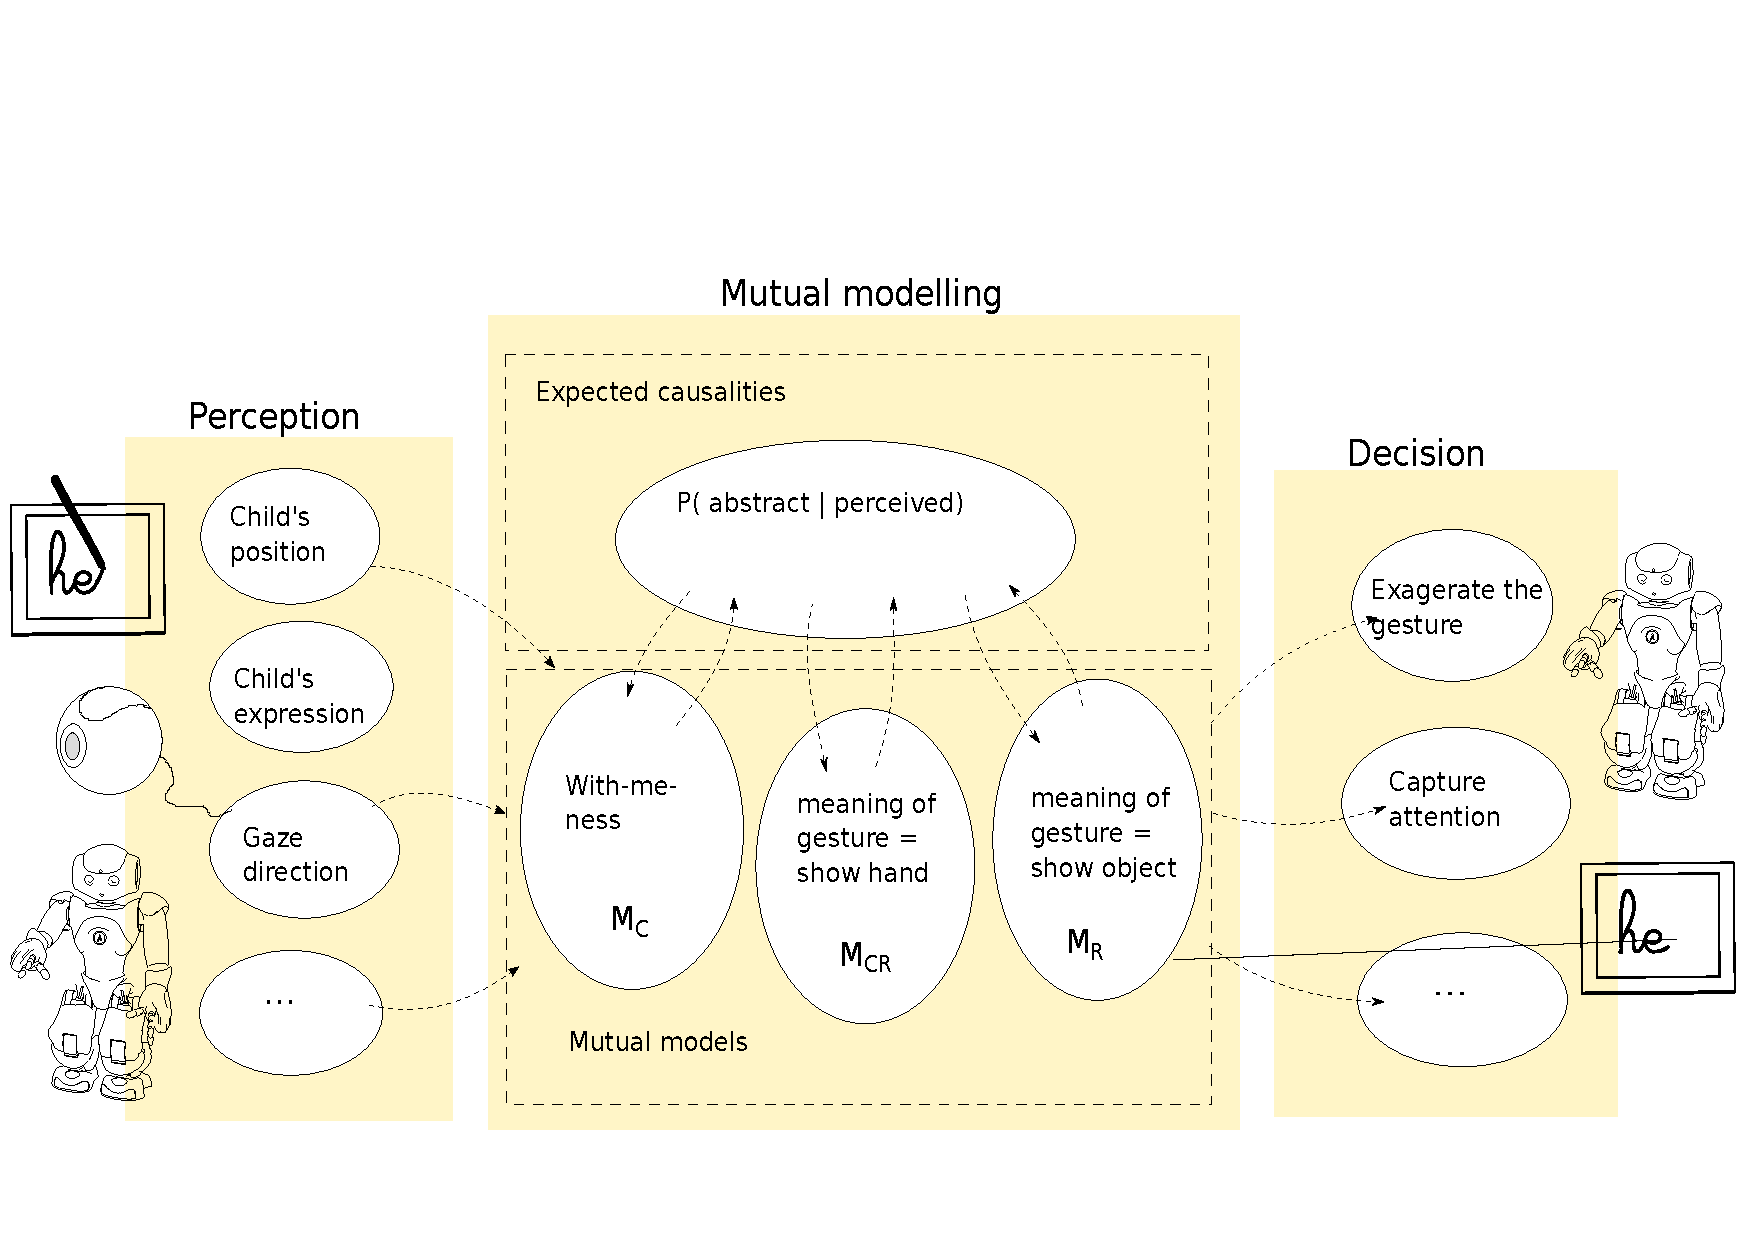
\includegraphics[width=1\columnwidth]{cognitive_archi}
\caption{\small\textbf{Overview of the cognitive architecture}. Yellow squares represent different main parts. White ellipses represent modules. We named in example some content of modules and illustrated possible devices used for perception and decisions with the context of the Cowriter Activity. We show a situation of miss-understanding : the child has a bad interpretation of the gesture of the robot. In order to repair this miss-understanding, a possible decision would be to exaggerate the movement. }
\label{cog}
\end{figure}
Our cognitive architecture for mutual modelling can be designed in three main parts. 
The \textbf{perception part} (see \ref{ssec:perception}) will regroup all the modules that measure the values of the perceived variables using sensors. 
These values are sent to the \textbf{mutual modelling part} (see \ref{ssec:mmm}) that updates in real-time models with measured values of perceived variables and deducts the value of abstract variables. Finally, the \textbf{decision part} (see \ref{ssec:decision}) contains all the modules associated to the control of the robot (and other active devices like tablets in CoWriter). These modules can read values given by mutual models in order to compute decisions. In the example of the CoWriter activity, these modules are given by the system that learns and generate letters, but we can add a module that generates micro-behaviour, another that decides to switch to a new activity (e.g. drawing with the robot),\dots. The following subsections explain in detail the content and operation of each part of the architecture. 

\subsection{Perception modules}
\label{ssec:perception}
The sensitive modules sensors to measure value of relevant perceived variables. While agent's gazes direction and facial expression can be used in any interaction, some additive variables can be specific of the activity: in CoWriter, a module takes inputs of tablets to compute the new state of robot's writing. It defines a sensitive module, and the value of the new state of the robot to write a letter defines a perceived variable. As well, the evaluation of the robot by the child via the feedback buttons defines another perceived variable provided by the modules of the activity. Other modules are independent of the activity: the system that estimates the target objects looked by the child provides additive information not directly used by the modules of the activity.  

\subsection{Mutual modelling modules}
\label{ssec:mmm}
Each perceived value measured by sensitive modules are associated with the model of an agent (or a $n^{th}$-order agent). Each mutual model can be designed as a module that knows the list of its associated perceived variables and watch if the value of one of these variables has been changed. 
An additive module knows all the expected causalities and computes the values of abstract variables. Some expected causalities can be empirically learned and other set by hands. 

\subsection{Decision making}
\label{ssec:decision}
We believe that the values of variables provided by mutual modelling will provide rich and useful information for decision making. Taking in account these values to elaborate decision should improve the realism and the efficiency of the robot in the interaction.
Just like the sensitive ones, the modules that take decision can be specific of the activity (in CoWriter, the choice of a new learning curve or the decision to suddenly make a big mistake), or can govern a general behaviour (for example the exaggeration of a miss-understood gesture). Some decisions can have a high impact on the progress of the interaction: to stop an activity and to switch to a new one can frustrate a child that was committed into the activity. The conditions to make such a decision are not directly assessable, but must be learned by the robot. In order to make these decision cautiously, we propose to start by a Wizard-of-Oz approach and to move towards an autonomous approach following these steps: 
\begin{enumerate}
\item \textbf{Wizard-of-Oz}: A human takes decisions; the robot learns
\item \textbf{Mixed-initiative}: The robot makes suggestions; a human agrees or disagrees
\item \textbf{Autonomous}: The robot makes decisions
\end{enumerate}



\section{Conclusion}

Educational HRI based on learning by teaching approach needs robot able to perform second-level mutual modelling. 
We introduced a new approach to implement mutual modelling into a cognitive architecture. We used the CoWriter activity
as an example of application, but our architecture could be easily generalised for any kind of interaction.
We believe that this step must be reached in other context of HRI, in order to develop higher realism of behaviours
and to improve the quality of interactions. 

%\section{The need for cog archi in educational robotics}
%way to represent the learners knowledge
%
%essential for logical reasoning, 
%explanation of concepts
%
%
%
%\section{Related Works}
%According to \cite{Vernon2011}, the term ``cognitive architecture'' aimed to unify theories of cognition on various issues such as attention, memory, problem solving, decision making, learning, across different disciplines including psychology, neuroscience and computer-sciences.
%Some architectures are based on philosophical theories, some on biological theories and others on psychological theories~\cite{Thorisson2012,Chong2009}.
%Often; they do not aim to tackle the same research problem. 
%For instance, often, biologically based cognitive architectures aim to mimic the human brain while psychological ones focus on cognitive processes.
%
%There exist two main families of cognitive architectures: the \textit{cognitivist} and the \textit{emegergentist} perspectives.
%
%\paragraph{The Emergent Perspective} covers developmental cognitive architectures.
%In these types of architectures, the model and the processes are learned from experience. 
%Thus, the knowledge is automatically acquired. 
%However, these architectures also assume a part of innate knowledge at first.
%These systems are often platform-sensitive but research here usually focuses on general frameworks of model acquisition in order to be reusable on other platforms. 
%The model and the process are often task and domain dependent and are linked to sensorimotor loops.
%The emergent cognitive architectures reflect in some way the morphology of the system. 
%In this category, we find for example the \textit{HAMMER} \cite{Demiris2005} or the \textit{ICub Cognitive architecture} \cite{Vernon2007}.
%
%
%\paragraph{The Cognitivist Perspective} considers the cognitive architectures as generic computational models neither domain, nor task-specific. 
%A human programmer or machine learning feed the system with knowledge making it more specific to a task or a domain.
%The system is composed of computational models of cognition that are  taken from various sources (i.e biology, psychology, philosophy).
%For the cognitivists, the cognitive processes are independent from the physical platform (increasing the generic aspect of the computational models).
%
%\textit{ICARUS}, belonging to this family of cognitive architectures \cite{LaChRo2005,Langley2006} is also grounded in cognitive psychology, and \textit{AI} (like \textit{BDI} \footnote{BDI : Belief, Desire, Intention logic, developed by \cite{bratman1987}}) aims at unifying reactive and deliberative (problem-solving) execution, as well as symbolic and numeric (utilities) reasoning. 
%Memory is organised into short vs long-term, and conceptual vs skill memory.
%ICARUS has several goals but focuses only on the one with highest unsatisfied priority.
%The skills that allow to achieve it are brought from long-term to short-term memory.
%If no skill is available, the system uses means-end analysis to decompose into sub-goals, and learns from this impasse.
%
%For instance, some architectures are based on a set of generic and symbolic rules, such as \textit{Soar} \cite{Laird2012}, based on the unified theory of cognition, or \textit{ACT-R} \cite{Anderson2005}. 
%Many of these architectures are based on the ``mind-is-like-a-computer'' analogy.
%
%\begin{table}
%	\begin{tabular}{p{0.5\linewidth} p{0.5\linewidth}} \hline
%		System 1 (old mind) (intuitive) & System 2 (new mind) (reflective) \\ \hline
%		Does not require working memory Autonomous &
%		Requires working memory Cognitive decoupling; mental simulation \\
%		Fast & Slow \\
%		High capacity & Capacity limited \\
%		Parallel & Serial \\
%		Non-conscious &	Conscious \\
%		Biased responses & Normative responses \\
%		Contextualized & Abstract \\
%		Automatic & Controlled \\
%		Associative & Rule-based \\
%		Experience-based decision making & Consequential decision making \\
%		Independent of cognitive ability & Correlated with cognitive ability \\ \hline
%		Evolved early  & Evolved late \\
%		Similar to animal cognition &	Distinctively human \\
%		Implicit knowledge  & Explicit knowledge \\
%		Basic emotions & Complex emotions \\ \hline
%	\end{tabular}
%	\caption{Properties of System 1 and System 2 from the Dual-Process Theories of cognition from \cite{Evans2013}.}
%	\label{fig:dual_system}
%\end{table}
%%\vspace{1cm}
%
%The Dual-process theory marries these two families of cognitive architectures \cite{Evans2013}: the cognitivist and the emergentist.
%This theory states that there exist two cognitive systems involved in cognition, one fast and intuitive (S1) and the other, slow and deliberative (S2).
%The table~\ref{fig:dual_system} summarizes different characteristics of these two subsystems.
%Underlying these two systems (S1 and S2), we see the two families of cognitive architectures (Emergent and Cognitivist).
%
%\textbf{Hybrid approaches} of cognitive architectures constitute the last family combining Emergent and Cognitivist approaches.
%Hybrid architectures combine both types of processing. \textit{CLARION}  \cite{Sun2003} is an example of such an architecture.
%Recently, other architectures have been proposed, focusing on memory \cite{baxter2013} or attentional processes and a sensori-motor approach \cite{demiris2006}.
%
%
%\section{Mutual Modelling towards a model for TOM}
%Subsubsection text here.
%
%
%
%%What is the primary outstanding challenge in developing and/or applying cognitive architectures to social HRI systems?
%\section{Challenges for Cognitive Architecture for Educational HRI}
%Mainly method of evaluation to prove the following concepts
%\begin{enumerate}[noitemsep]
%		\item Categorise and Understand: enable to build ontologies and to acquire semantic knowledge.
%		\item Have an episodic memory and reflective processes.
%		\item Use ontology in order to encode the knowledge for more flexibility and re-usability.
%		\item Enable to communicate decision and plans.
%		\item Integrate new sensors for physical perception of the world.
%		\item Enable embodied applications and expressions.
%		\item Integrate emotions in the cognitive process.
%		\item Enable generalisation and modularity.
%\end{enumerate}
%
%
%\section{Conclusion}
%The conclusion goes here.


%\section*{Acknowledgment}


%The authors would like to thank...






\bibliographystyle{IEEEtran}

\bibliography{biblio}

\end{document}


